% This file was created by matlab2tikz.
% Minimal pgfplots version: 1.3
%
%The latest updates can be retrieved from
%  http://www.mathworks.com/matlabcentral/fileexchange/22022-matlab2tikz
%where you can also make suggestions and rate matlab2tikz.
%
\documentclass[tikz]{standalone}
\usepackage{pgfplots}
\usepackage{grffile}
\pgfplotsset{compat=newest}
\usetikzlibrary{plotmarks}
\usepackage{amsmath}

\begin{document}
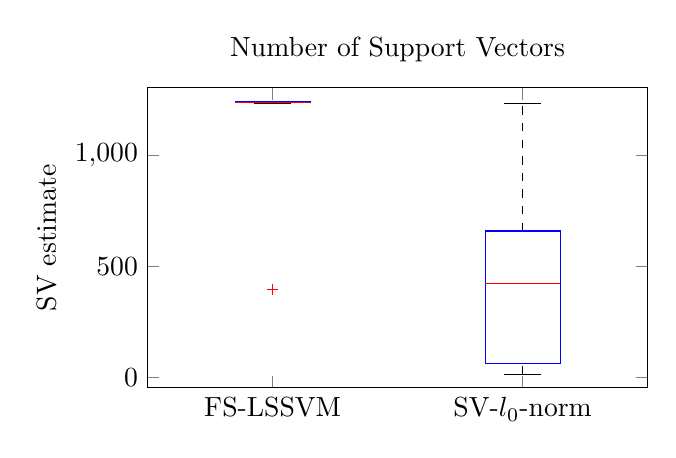
\begin{tikzpicture}

\begin{axis}[%
width=2.5in,
height=1.5in,
scale only axis,
unbounded coords=jump,
xmin=0.5,
xmax=2.5,
xtick={1,2},
xticklabels={{FS-LSSVM},{SV-$l_0$-norm}},
ymin=-46.4,
ymax=1304.4,
ylabel={SV estimate},
title={Number of Support Vectors}
]
\addplot [color=black,dashed,forget plot]
  table[row sep=crcr]{%
1	1241\\
1	1243\\
};
\addplot [color=black,dashed,forget plot]
  table[row sep=crcr]{%
2	660\\
2	1235\\
};
\addplot [color=black,dashed,forget plot]
  table[row sep=crcr]{%
1	1236\\
1	1237\\
};
\addplot [color=black,dashed,forget plot]
  table[row sep=crcr]{%
2	15\\
2	63\\
};
\addplot [color=black,solid,forget plot]
  table[row sep=crcr]{%
0.925	1243\\
1.075	1243\\
};
\addplot [color=black,solid,forget plot]
  table[row sep=crcr]{%
1.925	1235\\
2.075	1235\\
};
\addplot [color=black,solid,forget plot]
  table[row sep=crcr]{%
0.925	1236\\
1.075	1236\\
};
\addplot [color=black,solid,forget plot]
  table[row sep=crcr]{%
1.925	15\\
2.075	15\\
};
\addplot [color=blue,solid,forget plot]
  table[row sep=crcr]{%
0.85	1237\\
0.85	1241\\
1.15	1241\\
1.15	1237\\
0.85	1237\\
};
\addplot [color=blue,solid,forget plot]
  table[row sep=crcr]{%
1.85	63\\
1.85	660\\
2.15	660\\
2.15	63\\
1.85	63\\
};
\addplot [color=red,solid,forget plot]
  table[row sep=crcr]{%
0.85	1237\\
1.15	1237\\
};
\addplot [color=red,solid,forget plot]
  table[row sep=crcr]{%
1.85	425.5\\
2.15	425.5\\
};
\addplot [color=black,only marks,mark=+,mark options={solid,draw=red},forget plot]
  table[row sep=crcr]{%
1	396\\
};
\addplot [color=black,only marks,mark=+,mark options={solid,draw=red},forget plot]
  table[row sep=crcr]{%
nan	nan\\
};
\end{axis}
\end{tikzpicture}%
\end{document}